In this chapter I will describe obtained results on each test machine. I will show scheduling executed by task-affinity and effects on cache miss and 
task migration. 

The ideally scheduling that the developed patch should be perform is showed in Fig. TODO. I have said "ideally" because, as described in \cite{lcs}, it is 
impossible to perform this scheduling, because scheduling latency are not equal for each core and tasks should wake up in the same time, i.e. waves, don't
wake up never in the same time etc.. 

TODO fig schedule

As we can see, the scheduling proposed, should significantly improve throughput. To estimate this improvement we use the \textit{amdhal's law} \cite{lcs}:

\begin{equation}
       Speedup = (\frac{P_{1}}{S_{1}} + \frac{P_{2}}{S_{2}} + ... \frac{P_{n}}{S_{n}})^{-1} 
\label{eq:amdhal}
\end{equation}

In this chapter I will show the behaviour of task-affinity on different architectures. First of all, using \textit{trace}, we will check if expected 
scheduling is performed, after which we will analyze how optimization proposed influence performance and L1 and LLC miss rate of the application. 

%%%%%%%%%%%%%%%%%%%%%%%%%%%%%%%%%%%%%%%%%%%%%%%%%%%%%%%%%%%%%%%%%%%%%%%%%%%%%
\section{Intel Xeon}

\begin{figure}[htbp]
\centering
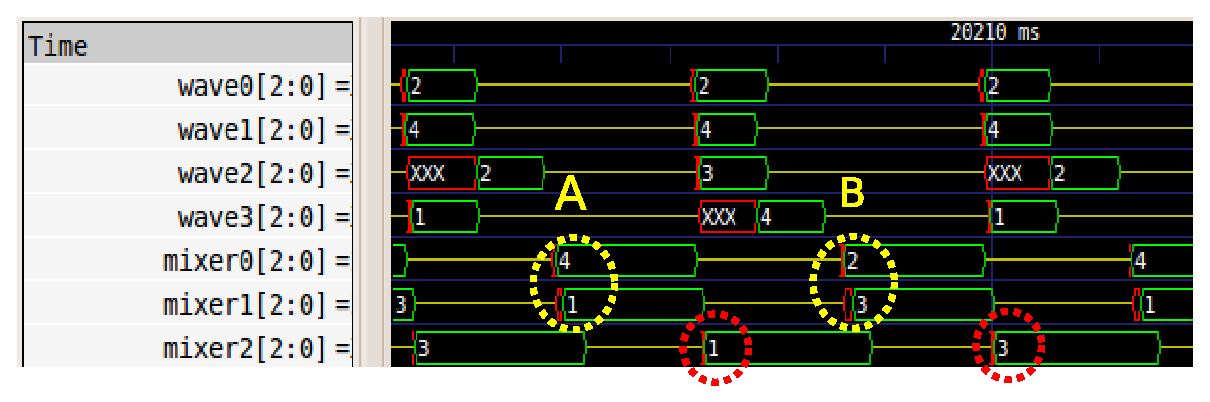
\includegraphics[width=\widefigure]{images/results_xeon/final_xeon.eps}
\caption{\figurecaption{trace TODO dire che sta a 32KB }}
\label{fig:trace_xeon}
\end{figure}

As we can see in Fig. \ref{fig:trace_xeon}, the scheduling performed is correct. We see that \textit{mixer2} can precede one of the waves and improve 
parallelism. We see that \textit{mixer0} chooses the best cpu in term of temporal locality, for example: in step A \textit{mixer0} chooses CPU4 and not 
CPU2, because on CPU2 was executed \textit{wave2}, therefore L1 cache could be dirty, instead on CPU4 the last task executed is \textit{wave1}, therefore 
L1 cache should be clean. Also in step B, it is possible to note how \textit{mixer0} take care about the last task executed on CPU4 choosing CPU2.

\begin{figure}[htbp]
\centering
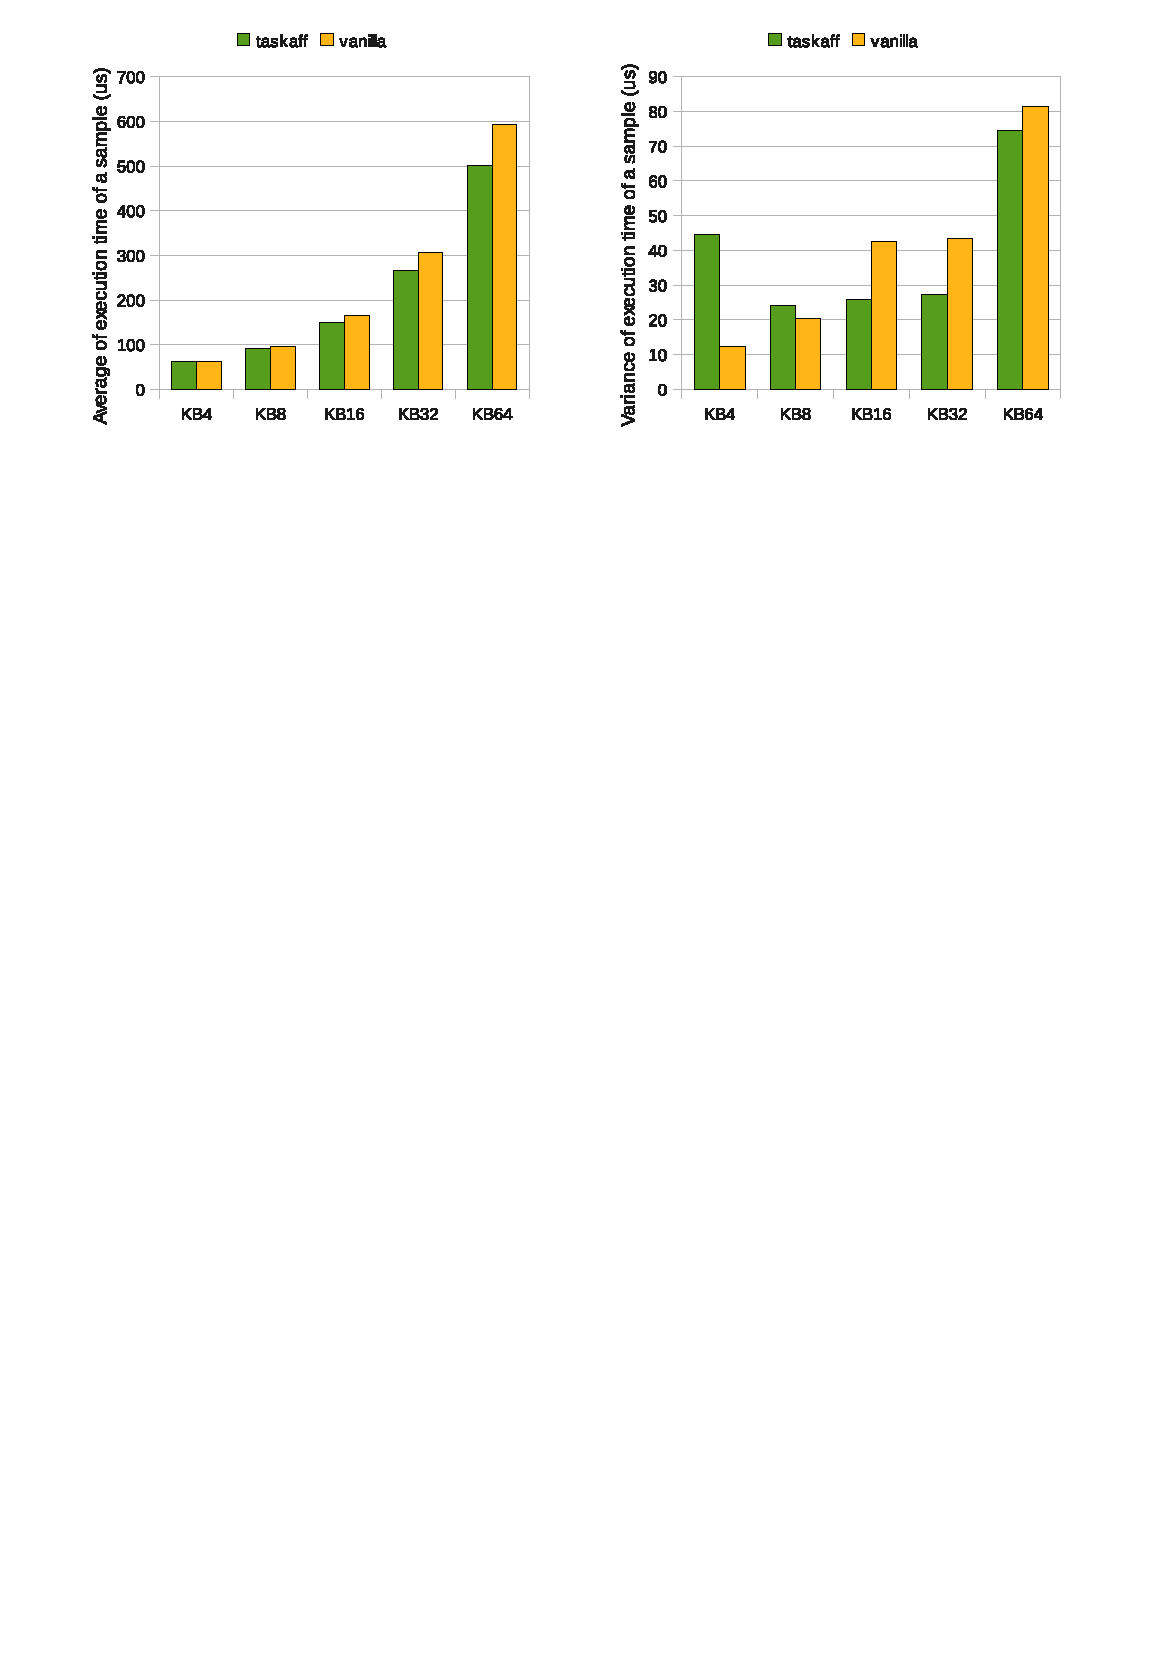
\includegraphics[width=\widefigure]{images/results_xeon/time_avg_var.eps}
\caption{\figurecaption{Average and Variance of execution time of a sample}}
\label{fig:time_avg_var_xeon}
\end{figure}

\begin{figure}[htbp]
\centering
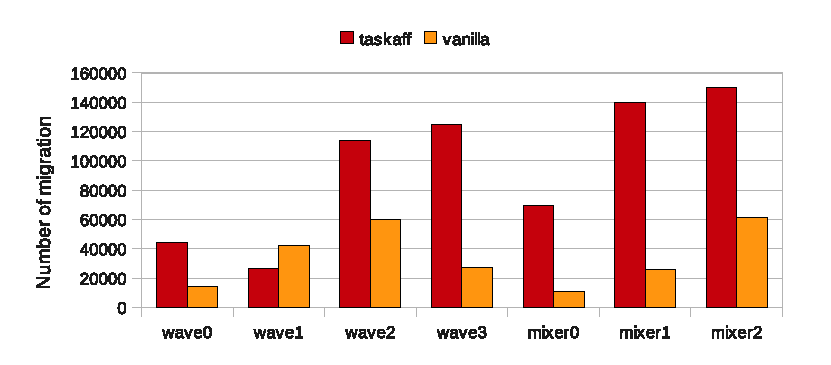
\includegraphics[width=\widefigure]{images/results_xeon/migration_xeon.eps}
\caption{\figurecaption{task migration on Xeon}}
\label{fig:migration_xeon}
\end{figure}

\begin{figure}[htbp]
\centering
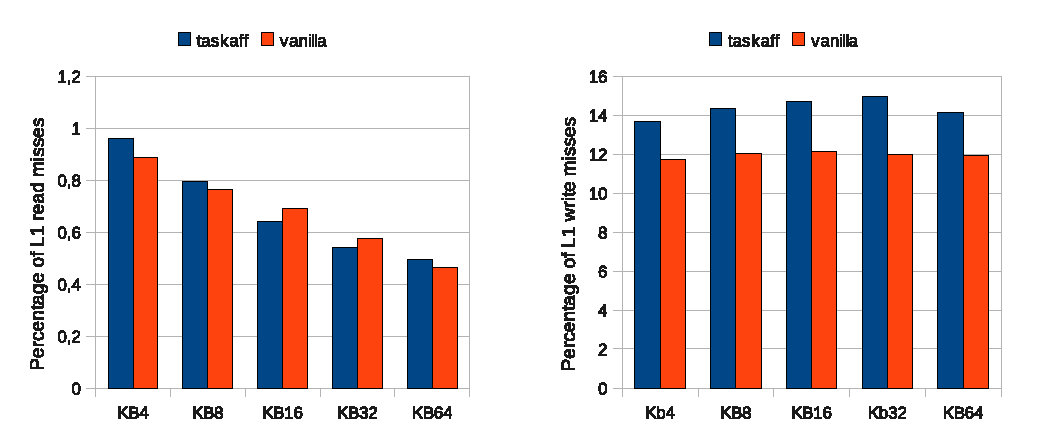
\includegraphics[width=\widefigure]{images/results_xeon/l1_load_store_xeon.eps}
\caption{\figurecaption{L1 Read and Write misses on Xeon}}
\label{fig:l1_load_store_xeon}
\end{figure}

\begin{figure}[htbp]
\centering
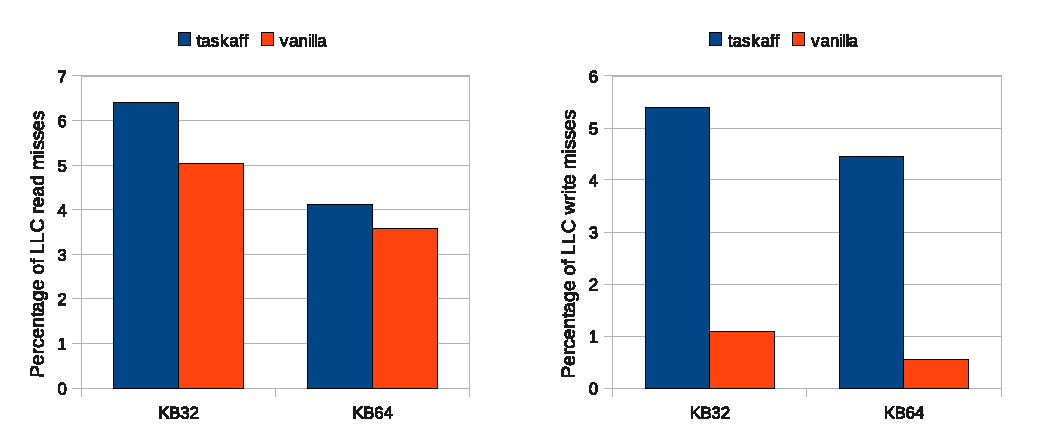
\includegraphics[width=\widefigure]{images/results_xeon/l2_load_store_xeon.eps}
\caption{\figurecaption{LLC Read and Write misses on Xeon}}
\label{fig:l2_load_store_xeon}
\end{figure}

\begin{table}[htbp]
\begin{center}
\begin{tabular}{l|c|c|c}
	\hline
	& Speedup on Xeon \\ \hline
	& taskaff & vanilla \\ \hline
	$4KB$  & 2.52 (3.13) \% & 2.09 (1.92)\% \\ \hline
	$8KB$  & 2.51 (3.14) \% & 2.13 (1.9)\% \\ \hline
	$16KB$ & 2.47 (3.14) \% & 2.15 (1.87)\% \\ \hline
	$32KB$ & 2.47 (3.12) \% & 2.22 (1.83)\% \\ \hline
	$64KB$ & 2.45 (3.12) \% & 2.38 (1.82)\% \\ \hline
\end{tabular}
\label{tab:speedup_xeon_i7}
\caption{Speedup obtained with task-affinity and with vanilla on Xeon.}
\end{center}
\end{table}

%%%%%%%%%%%%%%%%%%%%%%%%%%%%%%%%%%%%%%%%%%%%%%%%%%%%%%%%%%%%%%%%%%%%%%%%%%%%%
\section{Intel i7}

\begin{figure}[htbp]
\centering
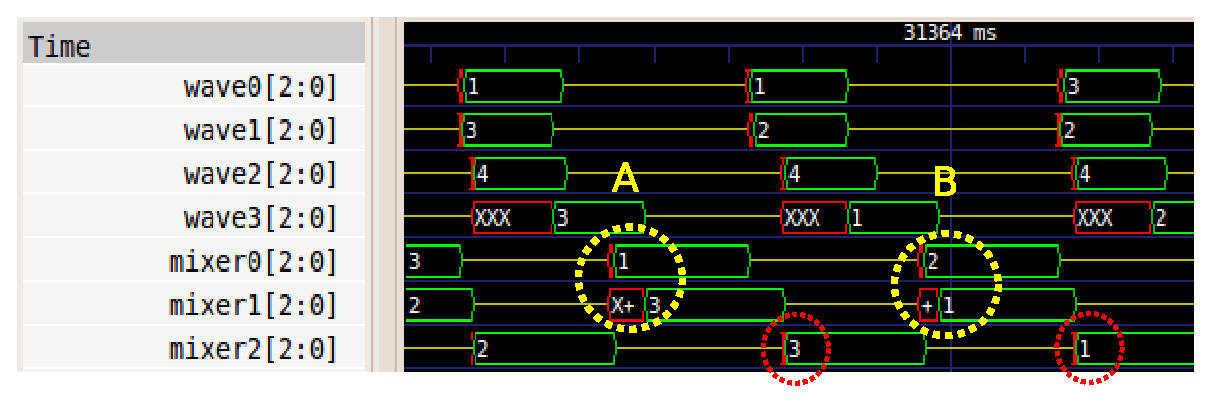
\includegraphics[width=\widefigure]{images/results_i7/final_i7.eps}
\caption{\figurecaption{trace TODO}}
\label{fig:trace_i7}
\end{figure}

Also in this case, Fig. \ref{fig:trace_i7}, the scheduling performed is correct. We can see how in step A and B mixers choose the correct CPUs according to
their task-affinity relationships.

\begin{figure}[htbp]
\centering
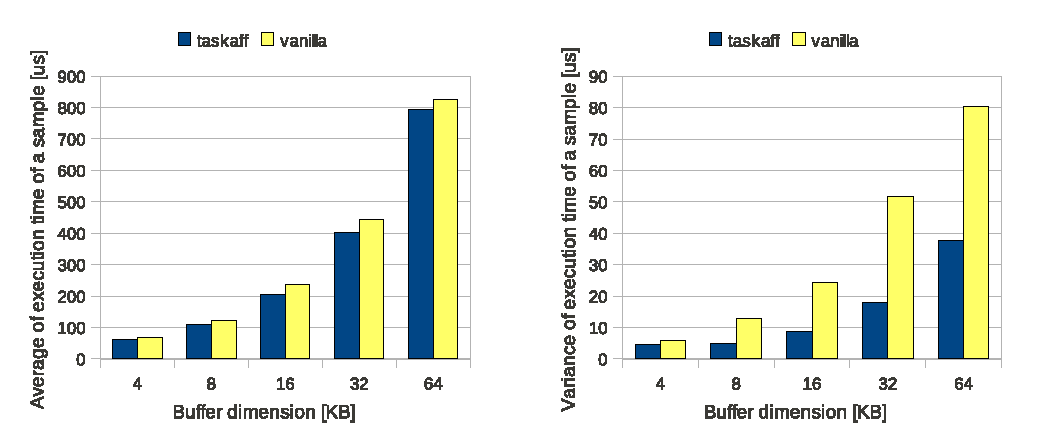
\includegraphics[width=\widefigure]{images/results_i7/time_avg_var_i7.eps}
\caption{\figurecaption{Average and Variance of execution time of a sample}}
\label{fig:time_avg_var_i7}
\end{figure}

\begin{figure}[htbp]
\centering
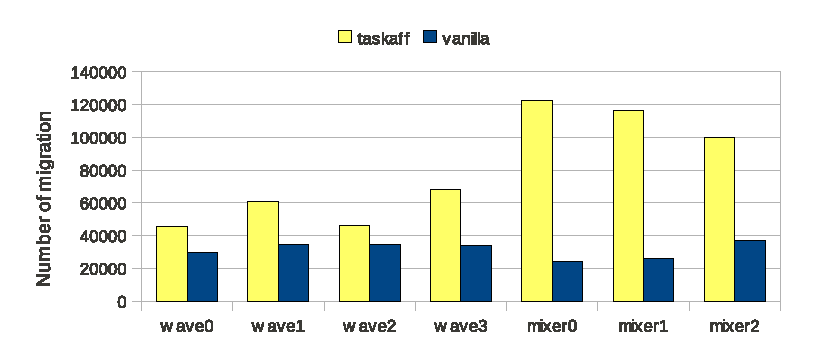
\includegraphics[width=\widefigure]{images/results_i7/migration_i7.eps}
\caption{\figurecaption{task migration on i7}}
\label{fig:migration_i7}
\end{figure}

\begin{figure}[htbp]
\centering
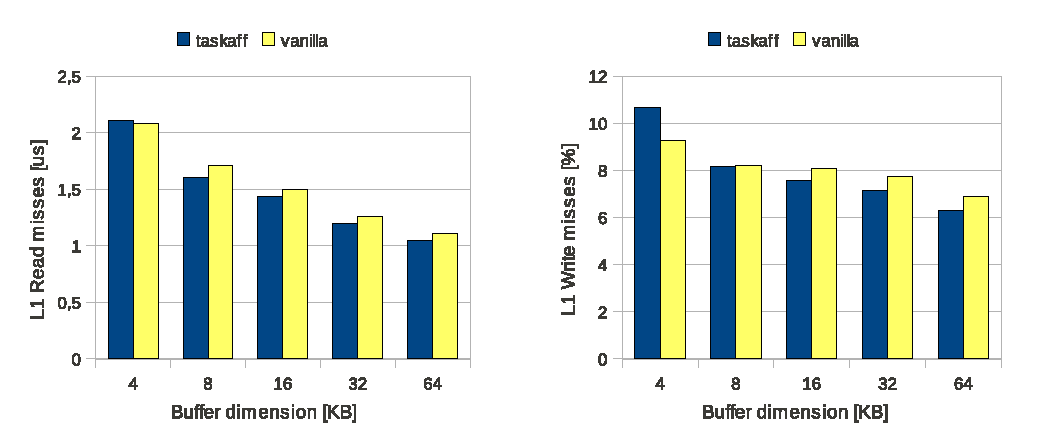
\includegraphics[width=\widefigure]{images/results_i7/l1_load_store_i7.eps}
\caption{\figurecaption{L1 Read and Write misses on i7}}
\label{fig:l1_load_store_i7}
\end{figure}

\begin{figure}[htbp]
\centering
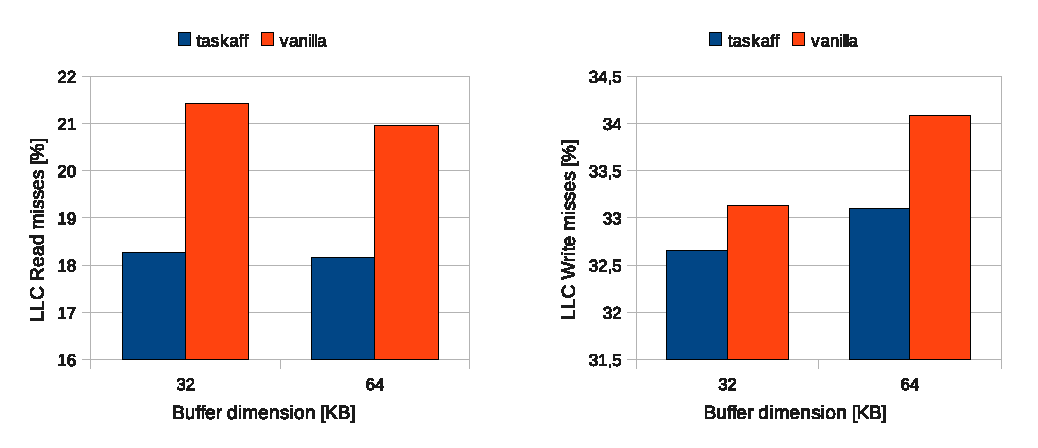
\includegraphics[width=\widefigure]{images/results_i7/l3_load_store_i7.eps}
\caption{\figurecaption{LLC Read and Write misses on i7}}
\label{fig:l2_load_store_i7}
\end{figure}

\begin{table}[htbp]
\begin{center}
\begin{tabular}{l|c|c|c}
	\hline
	& Speedup on i7 \\ \hline
	& taskaff & vanilla \\ \hline
	$4KB$  & 2.65 (3.48) \% & 2.32 (2.16)\% \\ \hline
	$8KB$  & 2.63 (3.4) \% & 2.24 (2.15)\% \\ \hline
	$16KB$ & 2.6 (3.38) \% & 2.18 (2.13)\% \\ \hline
	$32KB$ & 2.6 (3.33) \% & 2.27 (2.11)\% \\ \hline
	$64KB$ & 2.56 (3.27) \% & 2.28 (2.09)\% \\ \hline
\end{tabular}
\caption{Speedup obtained with task-affinity and with vanilla on i7.}
\label{tab:speedup_i7}
\end{center}
\end{table}

\newpage
%%%%%%%%%%%%%%%%%%%%%%%%%%%%%%%%%%%%%%%%%%%%%%%%%%%%%%%%%%%%%%%%%%%%%%%%%%%%%
\section{AMD}

\begin{figure}[htbp]
\centering
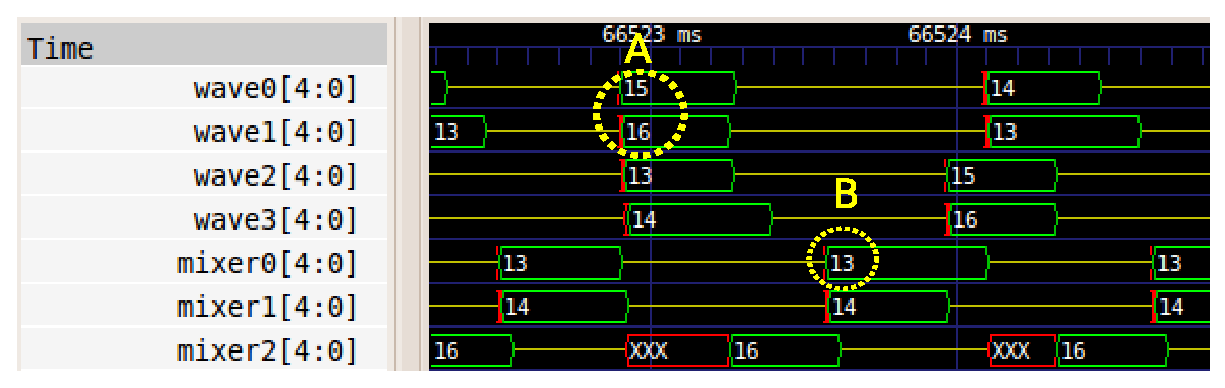
\includegraphics[width=\widefigure]{images/results_AMD/final_AMD.eps}
\caption{\figurecaption{trace TODO}}
\label{fig:trace_AMD}
\end{figure}

Unexplainably, task-affinity on this machine doesn't work. We can see in step B that \textit{mixer0} doesn't choose the correct CPU. AMD is a NUMA 
architecure and task-affinity patch it is developed for SMP architectures, therefore it could be necessary a revision of code in order to manage also 
NUMA architectures.

%%%%%%%%%%%%%%%%%%%%%%%%%%%%%%%%%%%%%%%%%%%%%%%%%%%%%%%%%%%%%%%%%%%%%%%%%%%%%
\section{Consideration on exeperimental results}

From previous graphics it is possbile to do some considerations:

\begin{description}

\item[throughput:] In both Intel Xeon and Intel i7, parallelism is improved. We can see in Fig \ref{fig:time_avg_var_xeon} an increment of throughput 
especially with 32 and 64KB, while at 4KB the increment is not very significant. This happens because at 4KB tasks are not well parallelized as we can see 
in Fig. TODO trace 4k
TODO giustifica speedup

\item[migrations:] Number of migration is greatly increased, this is not due to architectural details or different buffer dimensions. This fact happens 
because, at each sample, \textit{mixer0} and \textit{mixer1} and waves are excuted on the same CPUs. Since in the next sample waves are waken up during the 
execution of \textit{mixer0} and \textit{mixer1}, they must be scheduled on CPUs different from which that have executed them in the previous sample. 
For this reason, at each sample, waves are executed on different CPUs and, consequently, also other tasks are executed on different CPUs at each sample.

\item[cache misses:] Because of worsening of L1 and LLC cache misses, Fig \ref{fig:l1_load_store_xeon} \ref{fig:l2_load_store_xeon}, on Intel Xeon 
predictability of the application is degradated Fig. \ref{fig:time_avg_var_xeon}, especially using small buffer dimension such as 4KB or 8KB. LLC miss rate 
is greatly increased in task-affinity, because, as explained in the previous chapter, a core can access to data that are in caches of its own die, 
therefore if a task migrates frequently between two different dies, at each migration it will have to warm up LLC cache and a cache miss will occur. The 
same goes for L1 cache misses, also in that case a migration between CPUs that are in different dies increase L1 miss rates. Nevertheless with dimension 
greater than 8KB and especially greater than 32KB predictability is improved. This means that miss rates on Intel Xeon doesn't influence significantly 
predictability of the application. On Intel i7, instead, thanks to inclusive shared LLC, a core can access to data contained in all caches of other cores, 
consequently, L1 and LLC cache misses are reduced. The diminishing of cache misses impacts significantly on application predictability 
Fig.\ref{fig:time_avg_var_i7}.

\end{description}

TODO eviterei di metterla
 To explain this fact, it is necessary consider the overhead due to kernel 
functions: \texttt{push\_rt\_task} and \texttt{pull\_rt\_task}

